\documentclass[a4paper,12pt]{article}
\usepackage[utf8]{inputenc}
\usepackage[T1]{fontenc}
\usepackage{lmodern}
\usepackage{geometry}
\geometry{a4paper, margin=1in}
\usepackage{setspace}
\usepackage{tabularx}
\usepackage{lmodern}
\usepackage{xcolor}
\onehalfspacing
\usepackage{hyperref}

% Hyperref-Optionen, um Rahmen und Farben zu entfernen
\hypersetup{
    colorlinks=true,
    linkcolor=black, % Farbe der internen Links (z.B. im Inhaltsverzeichnis)
    urlcolor=blue,   % Farbe der URLs
    citecolor=black, % Farbe der Zitate
    filecolor=black  % Farbe von Datei-Links
}

\title{Projekthandbuch: PhileTipTip}
\author{Matthias Hochmuth}
\date{\today}

\begin{document}

\maketitle
\tableofcontents
\newpage

\section{Einleitung}

\section*{Über das Beispielunternehmen Philetairus Immobilien GmbH}
\addcontentsline{toc}{section}{Über das Beispielunternehmen Philetairus Immobilien GmbH}  

\begin{figure}[!h]
\centering

\includegraphics[width=4.5cm, height=4.5cm]{PhiletairusLogo}
\caption{Logo der Philetairus  Immobilien GmbH, }
\end{figure}

\begin{table}[ht]
    \centering
    \begin{tabularx}{\textwidth}{|l|X|X|} 
        \hline
        Firmenname & Philetairus Immobilien GmbH\\
        \hline
        Gesellschaftsform & GmbH\\
        \hline
        Branche & Immobilienindustrie\\
        \hline
        Gründungsjahr & 1979\\
        \hline
        Standorte & Wiesbaden(Hauptsitz), \\ Limburg an der Lahn, Mainz\\
        \hline
        Produzent oder Dienstleister & Dienstleister\\
        \hline
        Anzahl Mitarbeiter & 550\\
        \hline
    \end{tabularx}
    \caption{Steckbrief Philetairus  Immobilien GmbH}
    \label{tab:firmenSteckbrief}
\end{table}

\paragraph{Hauptdienstleistungen}

Die Philetairus Immobilien GmbH ist ein Komplettdienstleister im Bereich der Immobilienwirtschaft. Das Kerngeschäft umfasst die Verwaltung von Wohnungseigentum (WEG-Verwaltung) sowie die Miet- und Sondereigentumsverwaltung. \\

Weitere Dienstleistungen beinhalten technisches, kaufmännisches und infrastrukturelles Gebäudemanagement, Vermietungsmanagement, Erstellung der Betriebskostenabrechnungen sowie Hausmeisterservices.\\

\paragraph{Firmenziele}

Die Philetairus Immobilien GmbH strebt danach, einen umfassenden Service für die zu verwaltenden Immobilien zu bieten, der sowohl Eigentümer als auch Mieter zufriedenstellt. Ein weiteres Ziel ist die Förderung einer starken Kooperation der einzelnen Unternehmensbereiche, um einen zentralen Anlaufpunkt für alle Bedürfnisse der Auftraggeber zu bieten.\\

Die hier beschriebene Firma ist rein fiktiv und wurde nur für den Zweck der Habmann Abschlussarbeit erstellt und wurde im Rahmen dieses Moduls unverändert übernommen. \\
\newpage


\subsection{Projektbeschreibung}
Kurze Einführung in das Projekt, Zielsetzung und Nutzen.

\subsubsection{Einführung}

Das Projekt PhileTipTip zielt darauf ab, ein innovatives System für die Abteilung Außenarbeiten zu entwickeln. Dieses System soll in Form einer Android-App realisiert werden und dient als Kommunikationsbrücke zwischen Mietern/Eigentümern und der Grünflächenabteilung einer Immobilienverwaltung. Zusätzlich soll ein Administrations Tool für die Desktop Anwendung entstehen, die das erfassen von neuen Datensätzen für Mieter, Gebäude und Mitarbeiterdaten vereinfacht und vereinheitlicht. Für dieses Pionierprojekt sollen beide Komponenten der Erfassung von Meldungen für die Grünflächenabteilung dienen, aber perspektivisch soll mit diesem Projekt der Grundstein für eine umfassende Digitalisierung des gesamten Unternehmens gelegt werden.

\subsubsection{Zielsetzung}

Das Hauptziel des Projekts ist es, einen effizienten und benutzerfreundlichen Weg zu schaffen, um Meldungen über Probleme im Außenbereich von Immobilien zu erfassen, zu verwalten und zu bearbeiten. Insbesondere soll das System folgende Funktionen bieten:
\begin{itemize}
  \item  Ermöglichung der Erfassung von Meldungen durch Mieter und Eigentümer
  \item  Fokus auf Probleme im Zuständigkeitsbereich der Abteilung Außenarbeiten (z.B. Schädlingsbefall, Unkrautwuchs)
  \item  Effiziente Weiterleitung der Meldungen an die zuständige Abteilung
  \item  Verwaltung und Bearbeitung der eingegangenen Meldungen durch die Abteilung Außenarbeiten
\end{itemize}

\subsubsection{Nutzen}

Die Implementierung dieses Systems bringt mehrere Vorteile mit sich:
\begin{itemize}
  \item  Verbesserte Kommunikation zwischen Bewohnern und Immobilienverwaltung
  \item  Schnellere Reaktionszeiten auf Probleme im Außenbereich
  \item  Erhöhte Effizienz in der Bearbeitung von Meldungen
  \item  Bessere Übersicht und Nachverfolgbarkeit von Außenarbeiten
  \item  Steigerung der Zufriedenheit von Mietern und Eigentümern
\end{itemize}

\subsubsection{Kernfunktionen}

Die Android-App PhileTipTip wird folgende Kernfunktionen beinhalten:
\begin{itemize}
  \item  Benutzerfreundliche Oberfläche zur Erfassung von Meldungen
  \item  Möglichkeit zum Hochladen von Fotos zur besseren Dokumentation der Probleme
  \item  Kategorisierung der Meldungen (z.B. Schädlingsbefall, Unkrautwuchs)
  \item  Automatische Weiterleitung der Meldungen an die zuständige Abteilung
  \item  Statusverfolgung der Meldungen für Benutzer
  \item  Verwaltungsinterface für die Bearbeitung und Aktualisierung von Meldungen
\end{itemize}

\subsection{Zielgruppe}

Die primären Nutzer der App sind:
\begin{itemize}
  \item  Mieter von Immobilien
  \item  Eigentümer von Immobilien
  \item  Mitarbeiter der Abteilung Außenarbeiten in der Immobilienverwaltung
\end{itemize}

\subsection{Ziele des Projekts}

Durch die Entwicklung von PhileTipTip wird ein modernes, effizientes System geschaffen, das die Kommunikation und Problemlösung im Bereich der Außenarbeiten von Immobilien signifikant verbessert.

\newpage
\section{Projektorganisation}

\subsection{Auswahl der Projektstruktur}

Bevor mit der Planung des angestrebten Projekts begonnen werden kann, muss zunächst eine grundlegende Entscheidung über das Vorgehen und das Projektmanagementmethode getroffen werden. Da die verschiedenen Methoden bereits bei der Projektplanung teilweise bedeutende Unterschiede aufweisen, muss diese Entscheidung bereits vor der Planungsphase getroffen werden.

\subsection{Kurzer Vergleich gängiger Projektmanagementoptionen}
\label{subsec:pmstrukturen}

Grundsätzlich wird beim Projektmanagement zwischen drei Ansätzen unterschieden:\\

\begin{table}[ht]
    \centering
    \begin{tabularx}{\textwidth}{|l|X|X|} 
        \hline
        Klassisch & Linear Sequentiell. Erst wenn die Arbeiten eines Schrittes abgeschlossen wurden, wird mit dem nächsten begonnen. Die Abfolge und Abläufe der Schritte sind statisch und ein Abweichen vom Projektplan ist nicht ohne weiteres Möglich. Bei Projekten dieser Art wird viel Zeit auf eine sehr detailierte Vorplanung gelegt, die dann über fest definierte Meilensteine überprüft und gesteuert werden kann. Ein bekannter Vertreter dieses Ansatzes ist das Wasserfallmodell. \\
        \hline
        Agil & Inkrementell Iterativ. Während des Projektes wird das Endprodukt immer weiter verfeinert. Die Vorplanung bei Projekten dieser Art ist im Vergleich zum klassischen Vorgehen deutlich weniger detailiert. Viel mehr werden die Anforderungen in ständiger Kommunikation mit dem Kunden/Auftraggeber kontinuierlich überprüft und verfeinert, in der Regel nach dem Erreichen von Zwischenschritten (Inkrementen).  Ein bekannter Vertreter dieses Ansatzes ist Scrum. \\
        \hline
        Hybrid & Der Hybride Ansatz verbindet Elemente des Klassischen und des Agilen Projektmanagements um sich so die Vorteile beider Vorgehensweisen zu Nutze zu machen. Etwa indem die umfassende Projektstruktur klassisch aufgebaut ist um eine solide Struktur und klare Planbarkeit sicherzustellen, aber auf der Teamebene die Dynamik des 			agilen Ansatzes nutzt um bei der Erstellung des eigentlichen Projektprodukts flexibel agieren zu können. Eine Möglichkeit diesen Ansatz umzusetzen ist Prince2 (diese Methode bietet auch die Option rein klassisch vorzugehen)\\
        \hline
    \end{tabularx}
    \caption{Kurzübersicht Projektmanagementoptionen}
    \label{tab:pmOptionen}
\end{table}

\subsection{Agiles Vorgehen im Projekt}
\label{subsec:agilesVorgehen}

Eine etablierte Möglichkeit festzustellen, welches Vorgehen sich für ein konkretes Projekt eignet ist die Stacey Matrix.\\

\begin{figure}[!h]
\centering
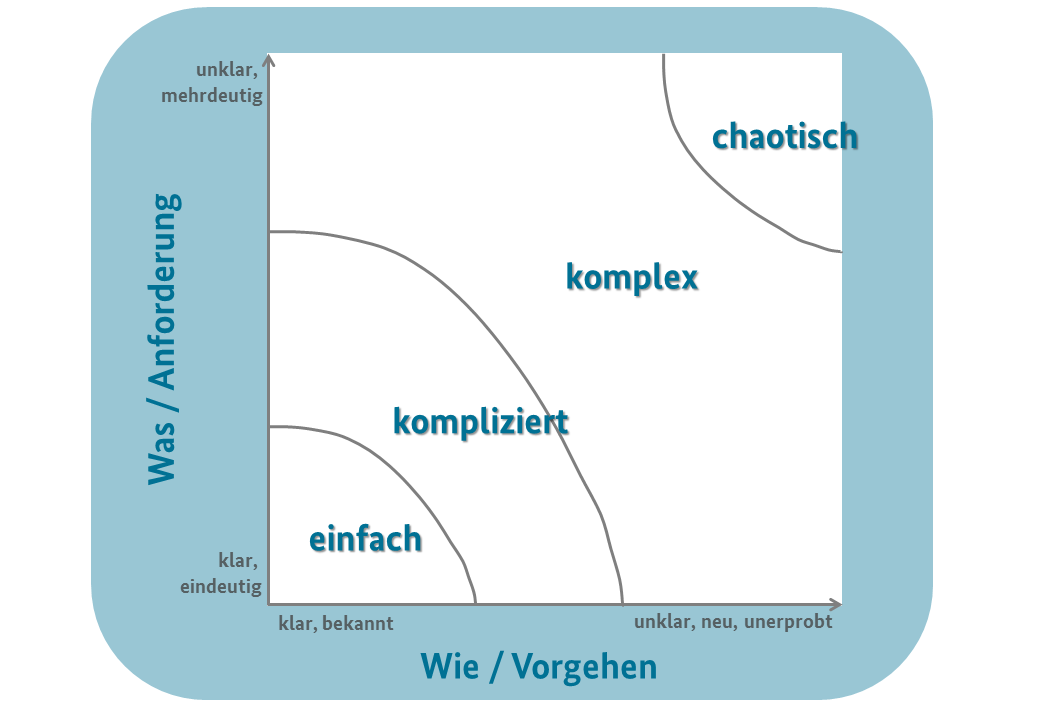
\includegraphics[width=6.24cm, height=4.32cm]{StaceyMatrix}
\caption{Stacey Matrix (\url{https://www.bva.bund.de/DE/Services/Behoerden/Beratung/Beratungszentrum/GrossPM/Wissenspool/_documents/Standardartikel/stda-stacey-matrix.html})}
\end{figure}

Im Bezug auf das geplante Projekt sind die Anforderungen noch nicht wirklich klar ausformuliert. Die Geschäftsführung hat eine Vision, eine grobe Idee und keinen klaren Katalog an sorgfältig definierten Anforderungen. Die Anforderungen sind also unklar.\\

Das Vorgehen an sich ist innerhalb des organisatorischen Ökosystems der Philetairus Immobilien GmbH unklar und unerprobt. Die IT Abteilung hat zuvor noch keine größeren Entwicklungsprojekte durchgeführt, daher ist auf diesem Gebiet wenig Erfahrung vorhanden und die Einbindung und  Einarbeitung der neuen Mitarbeiter kommt noch hinzu. Es gibt keine Erfahrungswerte innerhalb des Unternehmens auf die zurückgegriffen werden könnte, das Vorgehen ist daher unklar und unerprobt.\\

Basierend auf diesen Parametern ist dieses Projekt als Komplex einzuschätzen, daher ist ein agiles Vorgehen ratsam um der bestehenden Unklarheit möglichst flexibel zu begegnen und während des Projektes die geeigneten Methoden und Techniken zu erarbeiten. Für ein klassisches Vorgehen wäre eine langwierige Vorbereitungsphase notwendig, in der die genauen Anforderungen ermittelt werden müssten, bevor das Projekt überhaupt starten könnte.\\

Ein weiterer Vorteil des agilen Vorgehens in diesem Fall besteht in der zuvor beschriebenen Iterativen und Inkrementellen Vorgehensweise. So kann in regelmäßigen Abständen der Fortschritt überprüft werden und gegebenenfalls Anpassungen und Ergänzungen an den Anforderungen vorgenommen werden. Prinzipiell wäre das auch bei einem traditionellen Ansatz möglich, allerdings ist es dort mit einem größeren Aufwand verbunden einmal fixierte Projektanforderungen zu ändern .\\

Diese Flexibilität steht in direktem Zusammenhang mit der engen Einbindung der (in diesem Fall unternehmensinternen) Auftraggeber, die typisch für agiles Projektmanagement ist. Während die Auftraggeber bei klassischen Vorgehen konkrete Anforderungen zu Beginn des Projektes definieren und diese dann entweder zum Ende (oder zu festgelegten Meilensteinen) prüfen und abnehmen, stehen der Auftraggeber (oder dessen Vertreter) bei agilen Vorgehen in ständiger Kommunikation mit dem Entwicklerteam, prüfen die Zwischenprodukte (Inkremente) und beteiligen sich aktiv an der Anpassung und Aktualisierung der Anforderungen (zum Beispiel über das Product Backlog, siehe ~\ref{subsec:productGoalBacklog}).\\

Zu der Flexibilität des Vorgehens und des geringen Aufwands der Projektvorbereitung kommt ein weiterer Vorteil hinzu - die vergleichsweise hohe Anzahl der neuen Mitarbeiter, die durch die Erweiterung der IT Abteilung hinzugekommen sind. Diese sind noch nicht vollständig in die Unternehmensstrukturen integriert, auch hier bietet der agile Ansatz den Vorteil, da er auf flache Hierachien und Zusammenarbeit auf Augenhöhe setzt und die neuen Mitarbeiter somit schneller in das Ökosystem integriert werden können.\\

Aus diesen Gründen wurde der Entschluss gefasst, das Projekt agil anzugehen. Allerdings gab es von Seiten der Geschäftsleitungen einige Bedenken bezüglich eines rein agilen Vorgehens, weshalb weitere Überlegungen zur Projektstruktur angestellt wurden.\\
\subsection{Hybrides Vorgehen im Projekt}

Während die Stacey Matrix hilft das Projekt zu beurteilen und eine Entscheidung für klassisches oder agiles Vorgehen im Projekt zu treffen, gibt es andere Methoden und Hilfsmittel, den Projektkontext, nicht das Projekt als solches zu betrachten und einzuordnen. Eines davon ist das Agilometer:\\

\begin{figure}[hbt!]
\centering
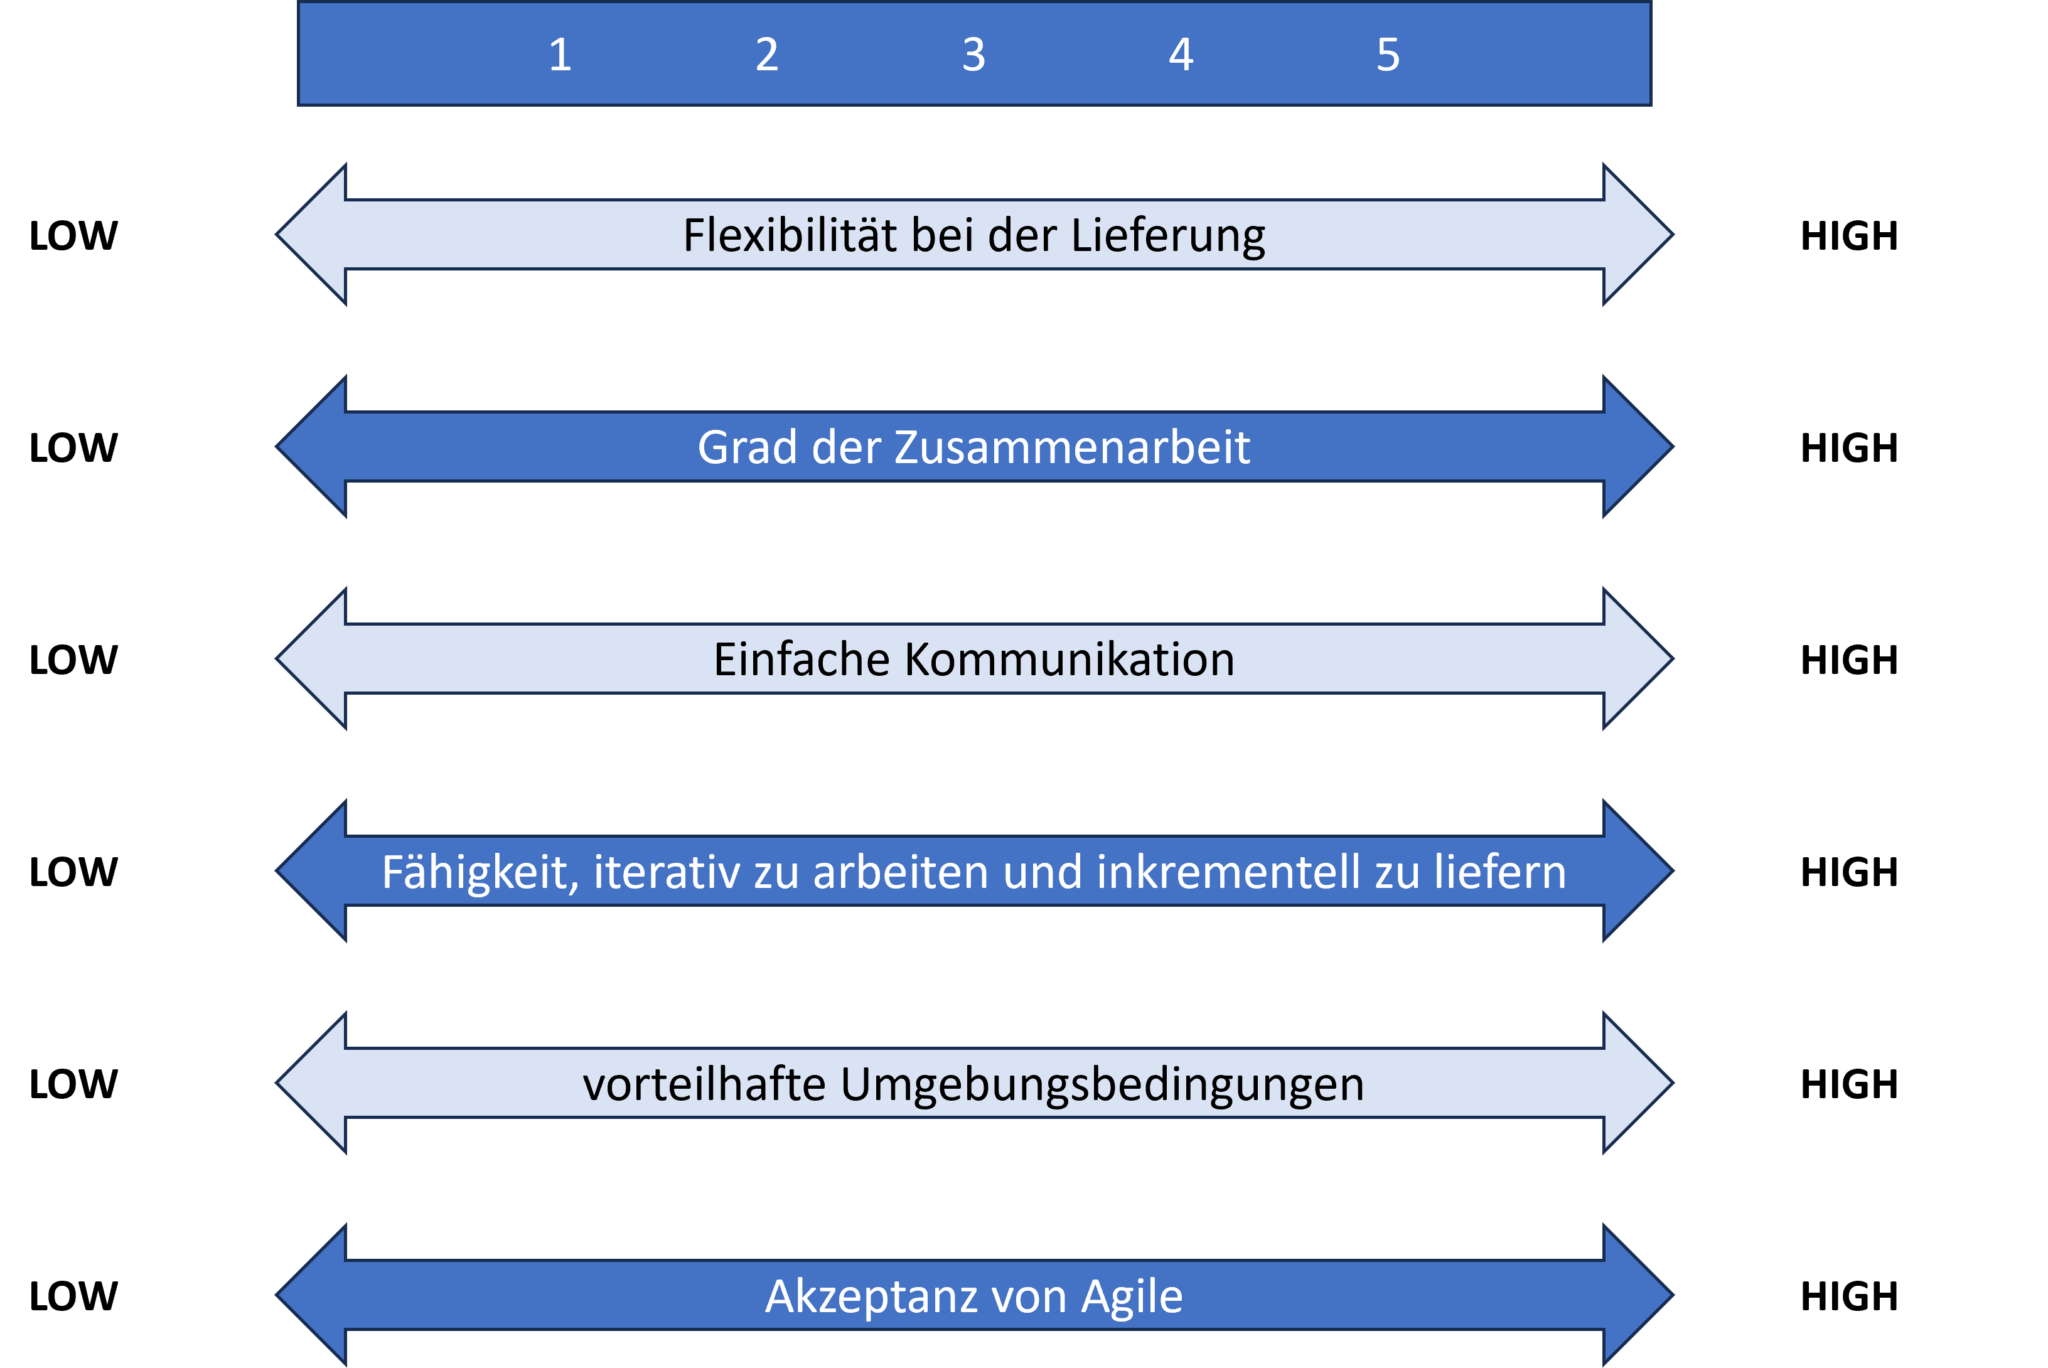
\includegraphics[width=9.69cm, height=6.48cm]{Agilometer}
\caption{Agilometer (\url{https://www.pureconsultant.de/de/agile/agilometer/})}
\end{figure}

Betrachtet man die Philetairus Immobilien GmbH, so ist der agile Reifegrad äußerst niedrig. Es gibt das Bestreben, zumindest auf der für das vorliegende Projekt relevanten Ebene agiler zu agieren, doch die mangelnde praktische Erfahrung bei der umsetzung von agilen Projekten, die immer noch bestehende Skepsis der Unternehmensführung und die große Anzahl von neuen Mitarbeitern in der ausführenden Abteilung deuten darauf hin, dass ein rein agiles Vorgehen keine sinnvolle Wahl wäre.\\

Ein klassisches Vorgehen nach dem Wasserfall- oder V-Modell wäre aufgrund der noch recht unkonkreten Zielsetzung des Projektes auch wenig praktikabel, da für diese Vorgehensweise mit Lasten- und Pflichtenheft die Anforderungen möglichst konkret und unmissverständlich formuliert werden müssen, bevor das Projekt initiiert werden kann.\\

Aus diesem Grund ist für das Vorhaben ein Hybrides Vorgehen, welches klassisches und agiles Vorgehen miteinander verbindet ideal. Für das agile Vorgehen fiel die Entscheidung auf Scrum (siehe ~\ref{subsec:agilesVorgehen}), den klassischen Rahmen soll Prince2 bilden.\\

Prince2 gibt klare Vorgaben, wie das Projektmanagementteam strukturiert sein sollte, für die Planung auf der Teamebene gibt es allerdings keine starren Richtlinien. Daher ist es möglich, ein hybrides Vorgehen zu wählen. Im Fall dieses Projekts wurde die Entscheidung für diese diese Variante getroffen: traditionelles Vorgehen auf der Entscheidungsebene und agiles Vorgehen auf der operativen Ebene. Somit bleibt ein großes Maß an Kontrolle erhalten, ohne die Vorteile des agilen Vorgehens zu sehr zu beschneiden.\\

Auf der anderen Seite definiert der Scrum Guide sehr genau die Rollen und Verantwortlichkeiten auf der Teamebene sowie das Vorgehen während der Entwicklung, die genaue Einbindung in die Unternehmensorganisation wird allerdings nicht konkret vorgegeben, somit ergänzen sich die beiden Vorgehensweisen, da es keine Überlappungen gibt, die Änderungen an einem der beiden Vorgehensmodellen nach sich ziehen und Kompromisse erfordern würden.\\

Ein weiterer Vorteil des Hybriden Vorgehens ist, dass gerade bei Prince2 durch die hohe Anzahl an Projektmanagementprodukten der Dokumentation von Erfahrungswerten ein hoher Wert beigemessen wird, die bei einem rein agilen Vorgehen eine untergeordnete Rolle spielt, wie es im bereits im agilen Mainifest niedergeschrieben wurde:\\

\textit{Funktionierende Software mehr als umfassende Dokumentation}\\

Zwar bedeutet das nicht, dass nicht dokumentiert werden sollte, allerdings wird dem einzelnen Inkrementen die in den Sprints erstellt werden ein höherer Stellenwert beigemessen. Das hybride Vorgehen ermöglicht es, diesem Gedanken gerecht zu werden, indem ein Großteil der Dokumentationsarbeit auf die Projektmanagementebene ausgelagert wird, wodurch das Entwicklerteam entlastet wird, aber dennoch eine umfassende Dokumentation der Erfahrungswerte gewährleistet wird.\\
\section{Anforderungsanalyse}

\subsection{Funktionale Anforderungen}

Die Funktionalen Anforderungen beantworten die Frage Was das Programm leisten soll.

\begin{itemize}
  \item Erfassung von Meldungen über Schädlingsbefall
  \item Speichern der Meldungen
  \item Anzeige und Sortierung dieser Meldungen
    \item Weiterleitung der Meldungen an die Grünflächenabteilung
    \item Benachrichtigungen an Nutzer über Bearbeitungsstatus
\end{itemize}

\subsection{Nicht-funktionale Anforderungen}

Die Nichtfunktionalen Anforderungen beantworten die Frage: Wie soll das Programm diese Anforderungen erfüllen?

\begin{itemize}
    \item Benutzerfreundlichkeit
    \item Performance und Sicherheit
  \item  Einfache Bedienbarkeit der App
  \item Leichte Wartbarkeit der App
  \item Leichte Erweiterbarkeit der App
  \item Zuverlässiges Funktionieren der App
  \item Datensicherheit und Datenschutz
  \item Schnelle Reaktionszeiten
  \item Niedriger Datenverbrauch im Mobilbetrieb
\end{itemize}

\subsection{Technische Anforderungen}
\begin{itemize}
    \item Android-Kompatibilität.
    \item Daten On-Premises, keine Cloud
\end{itemize}

\newpage

\subsection{User Stories}
\label{subsec:userStories}
\begin{table}[ht]
    \centering
    \begin{tabularx}{\textwidth}{|X|X|X|} 
        \hline
        Als [Rolle] & möchte ich [Funktionalität] & damit [Grund]\\
        \hline
        Mieter / Eigentümer & Schädlingsbefall / Unkrautbewuchs melden können & die Gärtner diesen zeitnah beseitigen\\
        \hline
        Landschaftsarchitekt & Mietermeldungen einsehen können & zu analysieren und Handlungsanweisungen geben zu können\\
        \hline
        Landschaftsarchitekt & Meldungen als Arbeitsanweisung an mein Team weiterleiten können & arbeiten zu koordinieren\\
        \hline
        Landschaftsarchitekt & einsehen können, woran mein Team gerade arbeitet & zu priorisieren und gegebenenfalls einzugreifen\\
        \hline
        Gärtner & einsehen können, wo ich arbeiten soll & den Einsatzort schnell finde \\
        \hline
        Gärtner & einsehen können, woran ich arbeiten soll & die Arbeit vorbereiten kann (passenede Herbi/Pestizide) \\
        \hline
        Abteilungsleiter Aussenarbeiten& einsehen können, woran die verschiedenen Teams gerade arbeiten & Arbeiten zu koordinieren und Absprachen mit den Landschaftsarchitekten halten zu können.\\
        \hline
        Abteilungsleiter Aussenarbeiten& die Meldungen über Befall und Bewuchs einsehen können & eventuelle Muster zu erkennen und großflächige Ausbreitung von Unkraut und Schädlingen zu verhindern.\\
        \hline
    \end{tabularx}
    \caption{Ausgewählte User Stories}
    \label{tab:userStories}
\end{table}
\section{App-Design}
\subsection{UI/UX}
\begin{itemize}
    \item Benutzeroberfläche (UI) für einfache Erfassung.
    \item Übersichtliche Navigation und Menüstruktur.
    \item Bild-Upload-Funktion zur Dokumentation.
    \item Klare, intuitive Navigation mit großen, leicht erkennbaren Buttons.
    \item Einsatz der Corporate-Farben: Dunkles Grün \textcolor[HTML]{23423d}{(23423d)} für Hauptelemente und Wheat \textcolor[HTML]{f5deb5}{(f5deb5)} für Hintergründe und Akzente.
    \item Integration des Webervogel-Logos als zentrales Designelement, z.B. als App-Icon und in der Kopfzeile.
    \item Bottom-Navigation-Bar mit maximal 4-5 Hauptkategorien für schnellen Zugriff.
    \item Einfacher Kamera-Button für direktes Fotografieren oder Auswahl aus der Galerie.
    \item Vorschau-Funktion mit Möglichkeit zur Bildbearbeitung (Zuschneiden, Drehen).
    \item Einfache Bedienbarkeit
    \item Step-by-Step Meldevorgang mit Fortschrittsanzeige.
    \item Autocomplete-Funktion für Adresseingabe und Problembeschreibung.
    \item Haptisches Feedback bei wichtigen Aktionen für bessere Nutzerinteraktion.
\end{itemize}

\subsection{Design-Richtlinien}

\begin{itemize}
    \item Konsistente Verwendung der Corporate-Farben 23423d und f5deb5 in allen UI-Elementen.
    \item Einheitliche Schriftart und -größen für optimale Lesbarkeit.
    \item Verwendung von Icons im Stil des Webervogel-Logos für eine harmonische visuelle Identität.
    \item Responsive Design für verschiedene Bildschirmgrößen und -orientierungen
\item Verwendung der offiziellen Google Icons für ein einheitliches Bild und bewährtes Design https://fonts.google.com/icons
\end{itemize}
\section{Technische Architektur}
\subsection{Systemarchitektur}

\subsubsection{Client-Server-Modell}

Die App PhileTipTip basiert auf einem klassischen Client-Server-Modell, bei dem die App als Client fungiert und über eine API mit einem zentralen Backend kommuniziert. Der Client (die App) ist für die Datenerfassung durch die Nutzer verantwortlich, während das Backend die Verarbeitung, Speicherung und Verwaltung dieser Daten übernimmt. Dieses Modell ermöglicht eine klare Trennung der Verantwortlichkeiten zwischen der Benutzeroberfläche und der Datenverarbeitung, was zu einer besseren Skalierbarkeit und Flexibilität führt.

\subsubsection{Integration der Datenbank}

Die MySQL-Datenbank ist fest in das Backend integriert und dient als zentrale Speicherinstanz für die erfassten Meldungen. Jede Anfrage des Clients, die eine Datenveränderung oder -abfrage erfordert, wird vom Backend an die Datenbank weitergeleitet. Über definierte API-Endpunkte können Nutzer der App Meldungen zu Schädlingsbefall oder Unkrautbewuchs erstellen und den Status dieser Meldungen abfragen. Gleichzeitig erlaubt das Backend der Grünflächenabteilung, auf diese Daten zuzugreifen, sie zu bearbeiten und den Bearbeitungsstatus zu aktualisieren.

\subsubsection{Backend und API}

Das Backend wird als Vermittler zwischen der App und der Datenbank fungieren. Es nimmt die Anfragen des Clients entgegen, verarbeitet sie und stellt die entsprechenden Daten bereit. Die API, die auf REST-Prinzipien basiert, stellt sicher, dass die Kommunikation zwischen der App und dem Server effizient und sicher erfolgt. Zu den wichtigsten Aufgaben des Backends gehören:

\begin{itemize}
    \item Verarbeitung von Nutzeranfragen: z.B. das Erstellen neuer Meldungen oder das Abrufen bestehender Einträge.
    \item Sicherheit und Authentifizierung: Schutz der Daten durch Zugriffskontrollen und verschlüsselte Kommunikation.
    \item Datenmanagement: Verwaltung und Speicherung der Daten in der MySQL-Datenbank sowie Sicherstellung der Datenintegrität.
\end{itemize}

Diese Architektur sorgt für eine flexible und robuste App, die auf wachsende Nutzerzahlen und Anforderungen skalierbar ist. Zudem ermöglicht sie eine klare Trennung zwischen Frontend (App) und Backend (Datenverarbeitung), was die Wartung und Weiterentwicklung der App erleichtert.

\subsection{Technologien}

\subsubsection{Android Studio und Java}

Die Entwicklung der App erfolgt in Android Studio, der offiziellen integrierten Entwicklungsumgebung (IDE) für Android. Android Studio bietet umfangreiche Tools für die Entwicklung, das Debugging und die Analyse der App-Performance. Als Programmiersprache wird Java verwendet, eine bewährte Sprache für die Android-Entwicklung. Java bietet eine große Entwickler-Community und umfangreiche Bibliotheken, die den Entwicklungsprozess beschleunigen und eine stabile, skalierbare App gewährleisten.

\subsubsection{MySQL-Datenbank}

Für die Verwaltung der Anwendungsdaten wird eine MySQL-Datenbank eingesetzt. MySQL ist ein weit verbreitetes relationales Datenbankmanagementsystem, das sich durch seine Zuverlässigkeit, hohe Performance und Skalierbarkeit auszeichnet. Die Datenbank speichert alle wichtigen Informationen, wie Benutzerdaten, Meldungen von Schädlingsbefall oder Unkrautbewuchs und deren Bearbeitungsstatus. Die Anbindung erfolgt über eine API, die die Kommunikation zwischen der App und der Datenbank ermöglicht.

\subsection{Schnittstellen}

\subsubsection{API zur Kommunikation zwischen Frontend und Backend}

Die Kommunikation zwischen dem Frontend (der Android-App) und dem Backend erfolgt über eine RESTful API. Diese API ermöglicht eine klare und strukturierte Interaktion zwischen den beiden Komponenten, indem sie Endpunkte bereitstellt, über die die App auf die vom Backend verwalteten Daten zugreifen kann. Jede Aktion, die von der App ausgeführt wird – sei es das Erfassen einer neuen Meldung von Schädlingsbefall oder das Abrufen des Status einer bestehenden Meldung – erfolgt über HTTP-Anfragen an die API.\\

Die wichtigsten API-Methoden umfassen:
\begin{itemize}
    \item POST: Zum Erstellen neuer Meldungen, die von Nutzern erfasst werden.
    \item GET: Zum Abrufen von Daten, wie z.B. dem Bearbeitungsstatus einer Meldung.
    \item PUT: Zum Aktualisieren von Daten, etwa wenn die Grünflächenabteilung den Status einer Meldung ändert.
    \item DELETE: Für das Löschen von nicht mehr relevanten Daten.
\end{itemize}

Die API ist dabei so konzipiert, dass sie sowohl eine hohe Performance als auch eine sichere Kommunikation gewährleistet. Dies erfolgt durch die Implementierung von HTTPS zur Verschlüsselung der Datenübertragung und einer Token-basierten Authentifizierung, die den Zugriff nur für berechtigte Nutzer und Systeme ermöglicht.

\subsubsection{Benachrichtigungssysteme}

Neben der reinen Datenkommunikation bietet die App ein Benachrichtigungssystem, das die Nutzer über den Status ihrer Meldungen informiert. Diese Benachrichtigungen werden durch das Backend ausgelöst, wenn bestimmte Ereignisse eintreten, wie z.B.:

\begin{itemize}
    \item Eingangsbestätigung einer Meldung: Sobald ein Nutzer eine Meldung abschickt, erhält er eine Bestätigung, dass die Daten erfolgreich erfasst wurden.
    \item Status-Updates: Sobald die Grünflächenabteilung eine Meldung bearbeitet oder den Status ändert, wird der Nutzer per Push-Benachrichtigung informiert.
    \item Erinnerungen: Falls eine Meldung über einen längeren Zeitraum unbeantwortet bleibt, können Erinnerungen an das Bearbeitungsteam oder die Nutzer gesendet werden.
\end{itemize}

Diese Benachrichtigungen werden über Firebase Cloud Messaging (FCM) versendet, das eine zuverlässige und effiziente Zustellung von Push-Benachrichtigungen an die Android-Geräte der Nutzer sicherstellt. So bleiben die Nutzer jederzeit über den Stand ihrer Meldungen informiert, ohne aktiv in der App nachsehen zu müssen.
\section{Implementierung}
\subsection{Quellcodeverwaltung und Projektorganisation}

\subsubsection{Versionsverwaltung mit Git}

Für die Versionskontrolle des Projekts kommt Git zum Einsatz. Git ermöglicht es dem Entwicklerteam, Änderungen am Code effizient nachzuverfolgen, neue Features in separaten Branches zu entwickeln und verschiedene Versionen der App zu verwalten. Durch die Verwendung von Git wird die Zusammenarbeit im Team vereinfacht und mögliche Konflikte bei der Integration von Codeänderungen minimiert.

\subsubsection{Projektmanagement mit Jira}

Die Projektplanung und -verfolgung erfolgt über Jira, ein führendes Tool für das agile Projektmanagement. Mit Jira können Aufgaben und Anforderungen in Form von Tickets angelegt, priorisiert und nachverfolgt werden. Das Tool bietet auch Funktionen zur Sprint-Planung, Fortschrittsüberwachung und Berichterstellung, was eine effiziente und transparente Verwaltung des gesamten Entwicklungsprozesses ermöglicht.

\subsection{Codierstandards}
\subsection{Best Practices und Namenskonventionen}

Die Entwicklung der App PhileTipTip folgt klar definierten Codierstandards, um die Lesbarkeit, Wartbarkeit und Skalierbarkeit des Codes sicherzustellen. Die Einhaltung dieser Richtlinien ermöglicht eine konsistente Struktur des Quellcodes, erleichtert die Zusammenarbeit im Team und minimiert potenzielle Fehlerquellen.

\subsubsection{Konsequentes Einsetzen der Objektorientierung und Entwurfsmuster}
Die App wird vollständig nach dem Prinzip der Objektorientierten Programmierung (OOP) entwickelt. Dies bedeutet, dass alle funktionalen Bereiche in Klassen und Objekte unterteilt werden, um die Wiederverwendbarkeit und Modularität zu gewährleisten. Zudem kommen bewährte Entwurfsmuster wie das Singleton-Pattern (für die zentrale Verwaltung der Datenbankinstanz) und das Factory-Pattern (zur dynamischen Objekterstellung) zum Einsatz, um typische Aufgabenstellungen effizient zu lösen und den Code robust und flexibel zu halten.

\subsubsection{Modularisierung und Anwendung der SOLID-Prinzipien}
Ein zentrales Element der Architektur ist die strikte Modularisierung des Codes. Jede Funktionalität wird in klar abgegrenzten Modulen implementiert, die für sich unabhängig getestet und weiterentwickelt werden können. Diese Trennung fördert die Wiederverwendbarkeit von Code und erleichtert Erweiterungen. Zusätzlich wird die Entwicklung konsequent an den SOLID-Prinzipien ausgerichtet:
\begin{itemize}
    \item Single Responsibility Principle (SRP):Jede Klasse erfüllt nur eine klar definierte Aufgabe.
    \item Open-Closed Principle (OCP):*Klassen und Module sind offen für Erweiterungen, aber geschlossen für Änderungen, um unnötige Anpassungen im bestehenden Code zu vermeiden.
    \item Liskov Substitution Principle (LSP): Objekte von Unterklassen können durch Objekte der Oberklasse ersetzt werden, ohne dass das Verhalten der Anwendung beeinträchtigt wird.
    \item Interface Segregation Principle (ISP): Schnittstellen werden klein und spezifisch gehalten, um unnötige Abhängigkeiten zu vermeiden.
    \item Dependency Inversion Principle (DIP): Abhängigkeiten werden auf Abstraktionen statt auf konkrete Implementierungen aufgebaut, um die Flexibilität des Codes zu erhöhen.
\end{itemize}

\subsubsection{Kommentar- und Formatierungsrichtlinien}
Um den Code für alle Entwickler verständlich und nachvollziehbar zu gestalten, werden klare Kommentar- und Formatierungsrichtlinien beachtet. Kommentare erklären nicht nur den Zweck des Codes, sondern auch komplexe Abläufe, Algorithmen oder wichtige Entscheidungen bei der Implementierung. Dabei wird insbesondere auf die Prägnanz und Relevanz der Kommentare geachtet.

Bei der Formatierung folgen wir gängigen Konventionen, wie:
\begin{itemize}
    \item Einheitliche Einrückungen (z.B. 4 Leerzeichen pro Ebene).
    \item Sinnvolle Benennung von Variablen und Methoden nach dem CamelCase-Format.
    \item Konsistenter Einsatz von Leerzeilen und Absätzen zur logischen Gliederung des Codes.
    \item Begrenzung der Zeilenlänge, um die Lesbarkeit auf verschiedenen Bildschirmen zu gewährleisten.
\end{itemize}

Durch diese Maßnahmen wird sichergestellt, dass der Code nicht nur funktional korrekt ist, sondern auch für andere Entwickler leicht zu verstehen und weiterzuentwickeln ist.

\subsection{Feature-Entwicklung}
Schwerpunkte und iterative Entwicklung.

\subsection{Tests}
\begin{itemize}
    \item Unit-Tests und UI-Tests.
    \item Teststrategie für die App.
\end{itemize}

\section{Qualitätssicherung}
\subsection{Testplan}
Zeitplan für Tests und Fehlerbehebung.

\subsection{Testumgebung}
Beschreibung der Geräte und Android-Versionen.

\subsection{Abnahmekriterien}
Anforderungen für den Produktivstart.
\section{Datenschutz und Sicherheit}
\subsection{Datenschutz}
Umgang mit personenbezogenen Daten, Speicherung und Weiterleitung der Meldungen.

\subsection{Sicherheitsrichtlinien}
Zugriffskontrollen, Verschlüsselung von Daten, Backup-Strategien.

\section{Deployment und Wartung}
\subsection{Veröffentlichung}
App-Release im Google Play Store, Versionierung und Updates.

\subsection{Wartungsplan}
Fehlerbehebungen, Patches und langfristige Weiterentwicklung.
\section{Risiken und Herausforderungen}
\subsection{Risikomanagement}
Identifikation potenzieller Risiken und Maßnahmen zur Risikominimierung.

\subsection{Notfallpläne}
Vorgehen bei schwerwiegenden Fehlern oder Ausfällen.
\section{Abschluss und Ausblick}
\subsection{Projektabschluss}
Kriterien für den erfolgreichen Projektabschluss.

\subsection{Zukunftsperspektiven}
Erweiterungsmöglichkeiten der App (z.B. zusätzliche Funktionen oder Plattformen).

\end{document}
